\documentclass{sig-alternate}

% some more configurations
%-- Package hyperref ------------------------------------------------------------------------------
\usepackage[
	plainpages=false, %Gibt an auf welcher Seite die pdf-Darstellung beginnt.
	pdfpagelabels,
	pdftex=true,
	breaklinks=true, %/false: Gibt an, ob Links umgebrochen werden duerfen.
	%linktocpage=true/false: im Inhaltsverzeichnis sind nur die Seitenzahlen links, nicht der Text
	colorlinks=true, %/false: Links werden eingefaerbt (Farben werden mit linkcolor, anchorcolor ... festgelegt)
	linkcolor=black, %Farbe des verlinkten Textes, Dokument-interne Links
	citecolor=black, %Farbe des verlinkten Textes, Links zum Literaturverzeichnis
	filecolor=black, %Farbe des verlinkten Textes, Links auf lokale Dateien
	urlcolor=black, %Farbe des verlinkten Textes, externe URLs
	%frenchlinks=true/false: Links werden als smallcaps, anstatt farbig dargestellt.
	menucolor=black
]{hyperref}

\hypersetup{
	pdftitle={GreenSubway},
	pdfauthor={Andreas Jahn, Stephan Sigg},
	pdfsubject={GreenSubway},
	pdfkeywords={GreenSubway},
	%pdfpagelayout={TwoColumnRight}
	%bookmarksnumbered=true,
	%bookmarksopen=true,
	%bookmarksopenlevel=1,
	%pdfpagemode=None % None, UseOutline, UseThumbs, FullScreen
}
\usepackage{balance}  % to better equalize the last page

\begin{document}
%
% --- Author Metadata here ---
%\conferenceinfo{WOODSTOCK}{'97 El Paso, Texas USA}
%\CopyrightYear{2007} % Allows default copyright year (20XX) to be over-ridden - IF NEED BE.
%\crdata{0-12345-67-8/90/01}  % Allows default copyright data (0-89791-88-6/97/05) to be over-ridden - IF NEED BE.
% --- End of Author Metadata ---

\title{Prediction of passenger density in underground Systems}

\numberofauthors{2} %  in this sample file, there are a *total*
% of EIGHT authors. SIX appear on the 'first-page' (for formatting
% reasons) and the remaining two appear in the \additionalauthors section.
%
\author{
% You can go ahead and credit any number of authors here,
% e.g. one 'row of three' or two rows (consisting of one row of three
% and a second row of one, two or three).
%
% The command \alignauthor (no curly braces needed) should
% precede each author name, affiliation/snail-mail address and
% e-mail address. Additionally, tag each line of
% affiliation/address with \affaddr, and tag the e-mail address with \email.
%
% 1st. author
\alignauthor
Andreas Jahn and Klaus David\\
       \affaddr{Kassel University}\\
       \affaddr{Wilhelmh\"oher Allee 73}\\
       \affaddr{Kassel, Germany}\\
       \email{\{andreas.jahn,david\}@uni-kassel.de}
% 2nd. author
\alignauthor
Stephan Sigg and Xiaoming Fu\\
       \affaddr{Goettingen University}\\
       \affaddr{Goldschmidtstr. 7}\\
       \affaddr{G\"ottingen, Germany}\\
       \email{\{stephan.sigg, fu\}@informatik.uni-goettingen.de}
% 3rd. author
% \alignauthor
% Klaus David\\
%        \affaddr{Kassel University}\\
%        \affaddr{Wilhelmh\"oher Allee 73}\\
%        \affaddr{Kassel, Germany}\\
%        \email{david@uni-kassel.de}
}

% Title
\maketitle

% Abstract
\begin{abstract}

This paper provides a provides a comparison between several prediction accounts in the area of the underground stations.

\end{abstract}

% Introduction
\section{Introduction}
\label{sec:introduction}

Underground transportation systems are big energy consumers and have significant impacts on energy consumptions at a regional scale~\cite{anderson_maximizing_2009}. 

So far the optimization of the energy efficiency of transportation equipments, e.g. trains have been considered. Optimization of the energy efficiency of the metro stations operations, however, is only minimally exploited.

But realizing savings in energy consumption are meaningful for two reasons:
(\textit{i})~Despite the relatively small percentage that can be gained with optimal management of one metro station compared to optimizing trains, the high numbers of metro stations in the underground transportation will yield large energy savings in overall terms. In other words, in the management of metro stations is a high multiplication factor that boosts each relative small saving at a station level to a high saving at a metro network level.
Moreover (\textit{ii}) the optimization of the energy efficiency of the metro stations involves much less investments than the ones that are usually applied to transportation means and equipments. Consequently is it possible to distributed the technology easily across the whole metro network, as well as other transportation systems and realize savings in short term.

For example all Barcelona (Spain) metro stations consumes 63,1 millions of kWh annually~\cite{TMB}. A relative small saving of, e.g. 5\% in the electricity consumption of one metro station, is equivalent to the electricity consumed in more than 700 households during one year.

The optimized management of stations and surroundings, such as ventilation, vertical transportation and lighting does have an impact.

An approach to optimize the energy efficiency and to realize energy savings is to
enable the station to control the surroundings, such as ventilation, vertical transportation and lighting "intelligent" according the current situation. 
A simple example of "intelligent" control could be the slowing down the frequency of the ventilation-fans of the station, when the count of passenger doesn't make full speed necessary.

To achieve the context aware behaviour of a metro station basically two parts are necessary. (i) A controller which calculate the appropriate actions. A controller which is adaptive on the basis of various environmental factors, forecasts and passenger occupancy was developed~\cite{guo_intelligent_2013}.
(ii) The environmental factors, and prediction must be available for the controller. 

Staying in the given example the controller needs be aware about the current count of passengers in order to decrease the fan frequency if possible. However, increasing the fan frequency is more complex. Since the decreasing of the fan frequency doesn't have an immediate effect for the air quality the fan frequency needs to be decreased in a appropriate time before the stations is abruptly crowed again. To guarantee the required air quality on every point in time, the ventilation needs to be controlled in a foreseen manner, i.e. controlled on the prospectively number of passenger in the station.

This paper presents an approach for predicting the prediction of number of passenger in the station.

The remainder of this paper is organized as follows. In Section~\ref{sec:stateOfTheArt} an overview of the related literature is given. Section~\ref{sec:dataAcquisition} focuses on the data acquisition and the experiments, followed by Section~\ref{sec:results}, the evaluation and results. Last, Section~\ref{sec:conclusion}, summarizes the results.


% State of the art
\section{State of the art}
\label{sec:stateOfTheArt}

Context prediction breaks the border from reaction on past and present stimuli to proactive anticipation of actions. 
Initiated by the pioneering work of Mayrhofer et al.~\cite{5013}, researchers have for about one decade now considered the prediction of context to enable pro-active context computing. 
Research directions spread from applications for context prediction~\cite{5035} over event prediction~\cite{5071}, architectures for context prediction~\cite{5001,5010,4027}, data formats~\cite{Prediction_Bannach_2010} and algorithms~\cite{Prediction_Intille_2006}. 
% Recent work focuses on three main challenges that
% \begin{enumerate}
% \item prediction is mostly limited to location
% \item no benchmarks and common data sets exist  
% \item no common development framework exists
% \end{enumerate}
% While there have been contributions targeting some of these challenges, we still see them as unsolved and in the following will further elaborate on these challenges.
Several authors have studied aspects of future context with the aim of enabling proactive behaviour in applications. 
Applications considered are diverse and range across basically all aspects of daily life. 
Still, the survey of Voigtmann and David shows that a great share of context prediction research so far concentrates on location prediction~\cite{Prediction_Voigtmann_2012}. 
Recently the research on location prediction tends to focus on new approaches for indoor location, e.g.~\cite{Prediction_Ruscher_2012,Prediction_Murao_2012} and the use of social networks as data source~\cite{Prediction_Zhang_2012}. 
However, although frequently criticised~\cite{5088}, most work on context prediction focuses location prediction.
Notable exceptions are considering, for instance, prediction to reduce energy consumption in sensor nodes by powering only those components that are likely needed in the near future~\cite{ContextAwareness_Gordon_2011}, prediction for the comptation of trust in other pervasive devices~\cite{2040} or also the prediction of tasks a user likely engage in next in order to adapt the user interface over several devices properly~\cite{5019}.
Further exmamples are the prediction of user intention in order to proactively plan tasks of a robot the human is interacting with~\cite{5830} and the popular smart home use-case in which mobility patterns and device usage of inhabitants are predicted~\cite{5163}.

Regarding algorithms for context prediction, diverse approaches from various fields spanning, for instance, time-series forecasting or pattern matching have been applied. 
Prominent examples for context prediction techniques are Markov predictors \cite{6013}, SOM prediction methods \cite{6016,5001}, the state predictor method \cite{5027,5001}, neural network approaches \cite{5027,2026}, Bayesian networks \cite{5027}, prediction based on the principal component analysis \cite{2097}, ARMA predictors \cite{5001} as well as Kalman filter methods \cite{2040}, Fuzzy-State Q-Learning~\cite{ContextPrediction_Feki_2007} or alignment-based prediction~\cite{4026}.

These approaches are applied and implemented for a given use-case mostly from scratch, however, few architectures for context prediction have been proposed that would allow a generic implementation of context prediction while utilising arbitrary of these prediction algorithms~\cite{4011,5001,5010}.

But Context prediction is just a mere building brick in the implementation and instrumentation of a holistic application case. 
It consideres the important but yet isolated task of inferring [....]


%%%%%%%%%%%%%%%%%%%%%%%%%%%%%%%%%%%%%%%%%%%%%%%%%%%%%%%%%%%%%%%%%%%%%%%%%%%%%%%%%%%%%%%%%%%%%%%%%%%%%%%%%%%%%%%%%%%%%%%%%%%%%%%%%%%%%%%%%%%%%%%%%%%%%%%%%%
%%%%%%%%%%%%%%%%%%%%%%%%%%%%%%%%%%%%%%%%%%%%%%%%%%%%%%%%%%%%%%%%%%%%%%%%%%%%%%%%%%%%%%%%%%%%%%%%%%%%%%%%%%%%%%%%%%%%%%%%%%%%%%%%%%%%%%%%%%%%%%%%%%%%%%%%%%
%%%%%%%%%%%%%%%%%%%%%%%%%%%%%%%%%%%%%%%%%%%%%%%%%%%%%%%%%%%%%%%%%%%%%%%%%%%%%%%%%%%%%%%%%%%%%%%%%%%%%%%%%%%%%%%%%%%%%%%%%%%%%%%%%%%%%%%%%%%%%%%%%%%%%%%%%%
%%%%%%%%%%%%%%%%%%%%%%%%%%%%%%%%%%%%%%%%%%%%%%%%%%%%%%%%%%%%%%%%%%%%%%%%%%%%%%%%%%%%%%%%%%%%%%%%%%%%%%%%%%%%%%%%%%%%%%%%%%%%%%%%%%%%%%%%%%%%%%%%%%%%%%%%%%
%%%%%%%%%%%%%%%%%%%%%%%%%%%%%%%%%%%%%%%%%%%%%%%%%%%%%%%%%%%%%%%%%%%%%%%%%%%%%%%%%%%%%%%%%%%%%%%%%%%%%%%%%%%%%%%%%%%%%%%%%%%%%%%%%%%%%%%%%%%%%%%%%%%%%%%%%%
\textbf{Continue from here: differentiate context prediction from anticipatory sensing, applications:  also browse last awarecast workshops for further related work}
%%%%%%%%%%%%%%%%%%%%%%%%%%%%%%%%%%%%%%%%%%%%%%%%%%%%%%%%%%%%%%%%%%%%%%%%%%%%%%%%%%%%%%%%%%%%%%%%%%%%%%%%%%%%%%%%%%%%%%%%%%%%%%%%%%%%%%%%%%%%%%%%%%%%%%%%%%
%%%%%%%%%%%%%%%%%%%%%%%%%%%%%%%%%%%%%%%%%%%%%%%%%%%%%%%%%%%%%%%%%%%%%%%%%%%%%%%%%%%%%%%%%%%%%%%%%%%%%%%%%%%%%%%%%%%%%%%%%%%%%%%%%%%%%%%%%%%%%%%%%%%%%%%%%%
%%%%%%%%%%%%%%%%%%%%%%%%%%%%%%%%%%%%%%%%%%%%%%%%%%%%%%%%%%%%%%%%%%%%%%%%%%%%%%%%%%%%%%%%%%%%%%%%%%%%%%%%%%%%%%%%%%%%%%%%%%%%%%%%%%%%%%%%%%%%%%%%%%%%%%%%%%
%%%%%%%%%%%%%%%%%%%%%%%%%%%%%%%%%%%%%%%%%%%%%%%%%%%%%%%%%%%%%%%%%%%%%%%%%%%%%%%%%%%%%%%%%%%%%%%%%%%%%%%%%%%%%%%%%%%%%%%%%%%%%%%%%%%%%%%%%%%%%%%%%%%%%%%%%%
%%%%%%%%%%%%%%%%%%%%%%%%%%%%%%%%%%%%%%%%%%%%%%%%%%%%%%%%%%%%%%%%%%%%%%%%%%%%%%%%%%%%%%%%%%%%%%%%%%%%%%%%%%%%%%%%%%%%%%%%%%%%%%%%%%%%%%%%%%%%%%%%%%%%%%%%%%

We see a great potential for the use of context prediction in applications to enable sustainability, e.g. applications for energy efficiency. 
An important building block for this is the prediction of user preferences. 
Since preference settings in many applications tend to be complicated and have important implications, for example on the user's privacy, predicting the user's preferences was shown to solve the problem of too lax preference settings~\cite{Prediction_Bigwood_2012}. 
Also, important to enable applications for sustainability and energy efficiency, is the prediction of user routine, e.g.~\cite{Prediction_Seiter_2012}.    

Secondly, regarding missing benchmarks and data sets, although utilized by numerous algorithms, a comprehensive comparison of their strengths and weaknesses on benchmark data sets is yet missing. 
To raise context prediction to a professional level at which it might be integrated in commercial applications, we need to establish common, widely accepted data sets, develop and disseminate accepted benchmarks and provide more general description of algorithmic performance not only restricted to specific applications but to a whole class of applications utilising input data with similar properties. 
One promising approach is to utilize data that users share over social networks~\cite{Prediction_Zhang_2012}.

And last, although, several authors have considered architectures for context prediction~\cite{5001,4027,5010}, a common methodology or platform has not yet crystallised. 
Application developers are forced to start from scratch. One reason for this is that previous authors seldom provided usable sources of their applications that could be extended. 
In order to foster the integration of context prediction into applications, support for application developers has to be greatly improved. 

%% TODO: Add further literature and story
%% TODO: Add Awarecast 2013 papers.
%% TODO: Include also:
\cite{Prediction_Kasteren_2008,Prediction_Tenorth_2009}

% dataAcquisition
\section{Data Acquisition}
\label{sec:dataAcquisition}

The prediction is based on occupancy data gathered in a metro station. First some facts regarding the metro station will be given. Subsequently the data acquisition will be explained.

\subsection{Line Station}
\label{subsec:lineStation}

In this section the "station" is described. First the word "station" in the area of metro networks needs to be defined.

A metro network is composed by one or more metro lines. Each line has a fixed railway with a given number of stops to allow people to get on or off the trains by means of a platform: each of these stops is called "line station". A "metro station" is the concept that represents the point in space through which a passenger gets underground and into a line station. Metro station and line station can be the same physical entity, but it is possible that there are some "metro stations" that receive two or more "metro lines" in different platforms, and have therefore, two or more "line stations" within.

The data, used in this work, are gathered in line station in Passeig de Gr\`{a}cia - Line~3~(PdG-L3) in Barcelona. Passeig de Gr\`{a}cia~(PdG) is a station in the metro network of "Transports Metropolitans de Barcelona"~(TMB) and lies in a very iconic and touristic part of Barcelona. Some of the most popular buildings designed by Antoni Gaudi are in the proximity (Casa Batll\`{o}, Casa Mil\`{a}), as well as the city's most renown and exclusive boutiques.
The metro station is a historic icon of the Barcelona metro network. First opened in December of 1924, as a (line) station for Line~3, nowadays PdG holds three different line stations: L2, L3, and L4. The stations were built in three different periods and using different construction technologies in each of the premises (contemporary to the building periods). All line stations station has been refurbished a few times since 1924 and new equipment has been added recently.

Passeig~de~Gr\`{a}cia - Line~3~(PdG-L3) turns out to be representative for many station within TMBs metro network. Table~\ref{?} depicts the statistical reasons behind this~\cite{TMB}. Furthermore PdG-L3 is a crowded station which have low-rate usage hours as well. This provides a wide range of data which allows to test with very busy peak hours as well as with off-peaks. Figure~\ref{fig:PdG-L3_platforms} depicts the platforms of PdG-L3.

\begin{figure}[htb]
  \centering
  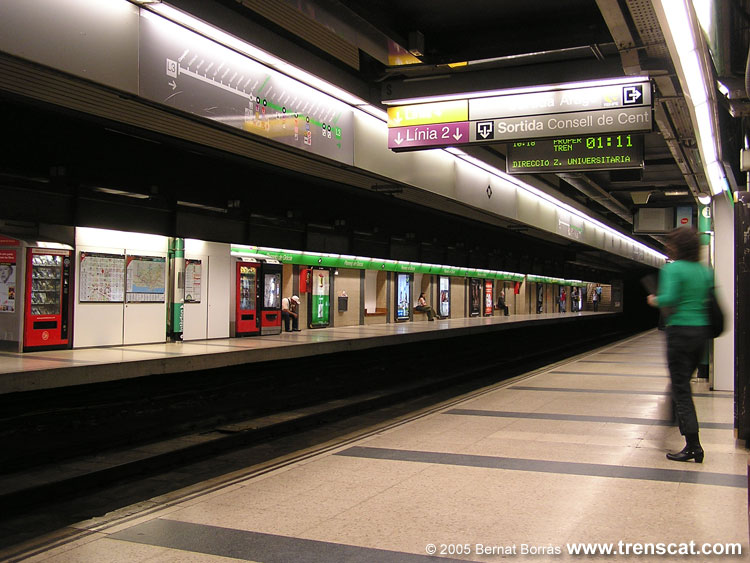
\includegraphics[width=\linewidth]{PdG-L3_platforms.jpg} 
  \caption{PdG-L3 Plattforms. \cite{TMB}}
  \label{fig:PdG-L3_platforms}
\end{figure}

The line station PdG-L3 consists of several public spaces: halls, transit areas, accesses to the platforms, and platforms. Furthermore there are private spaces such as technical rooms or staff dependencies. The private spaces are not part of the investigation in this work. Figure~\ref{fig:PdG-L3_schematic} depicts the line station schematic where the accesses to platforms are highlighted in red.

\begin{figure}[htb]
  \centering
  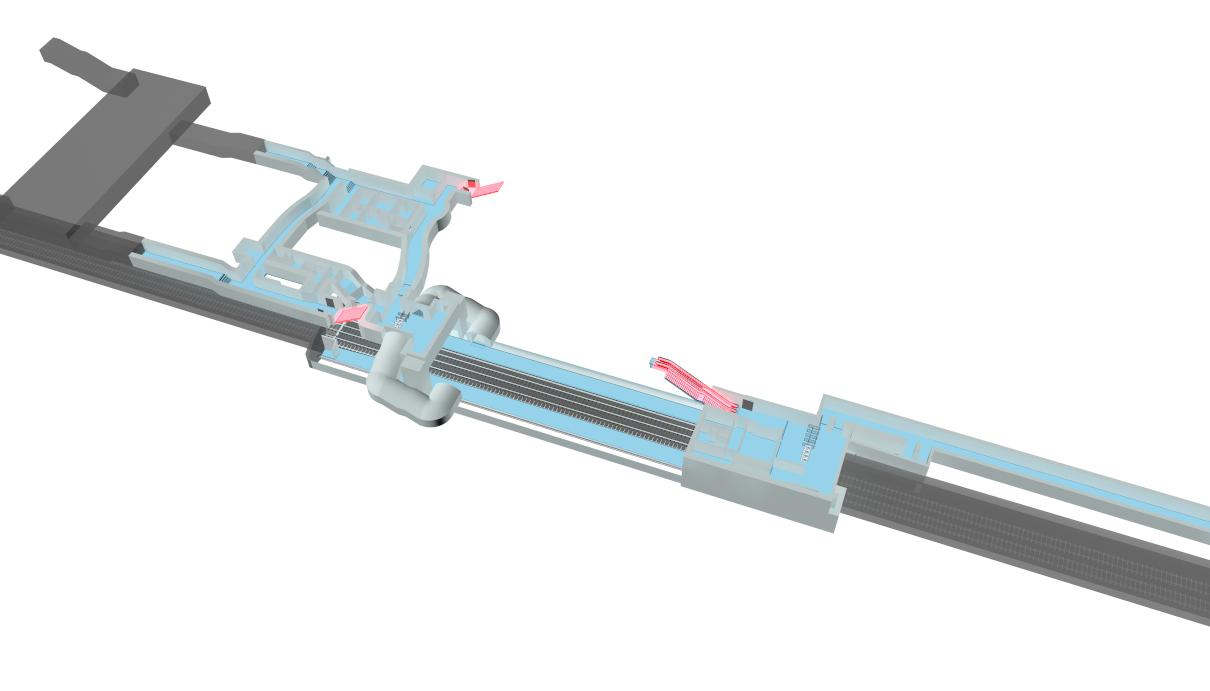
\includegraphics[width=\linewidth]{PdG-L3_schematic.jpg} 
  \caption{Schematic representation of PdG-L3. The accesses to platforms are highlighted in red. \cite{TMB}}
  \label{fig:PdG-L3_schematic}
\end{figure}

The public spaces are equipped with a Closed Circuit Television~(CCTV) for security reasons. The cameras of the CCTV-system provide images which contains the information how many people are on a dedicated time on a dedicated place. To gather these information the images needs to be processed. In the following the processing of the camera images is described in short.

\subsection{Data collecting}
\label{subsec:data}

The Data are gathered via CCTV. The CCTV images are stored on a video recorder. A crowd density estimator processes the images and returns the number of passengers on this image. The number of passenger are saved in a database together with a timestamp and the location. For privacy reasons the images are not saved over a longer time period. Figure~\ref{fig:crowdDensityEstimator} depict the processing chain.

\begin{figure}[htb]
  \centering
  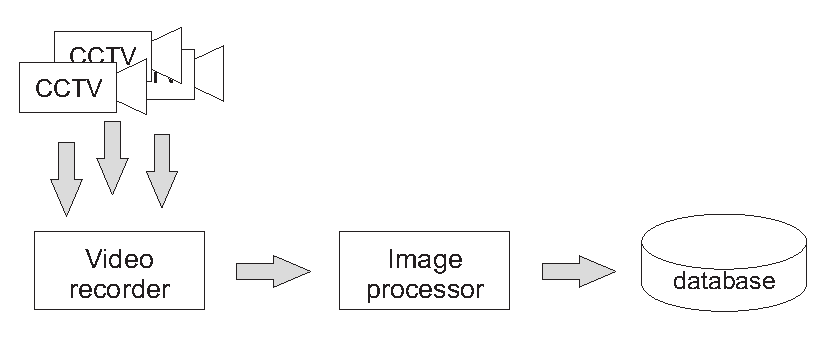
\includegraphics[width=\linewidth]{imageProcessing.pdf} 
  \caption{Gathering number of people out of the camera images}
  \label{fig:crowdDensityEstimator}
\end{figure}

% Results
\section{Results}
\label{sec:results}

This section focuses on the evaluation and the results. First the evaluation of the recorded sensor data is shown. Subsequently the results are presented and discussed.

\subsection{Evaluation}
\label{subsec:evaluation}

The evaluation analyses the prediction occupancy and provides a measurement in order to depict the prediction performance. The evaluation in detail is depicted in the following.

\subsubsection{Performance measurement}
\label{subsubsec:performanceMeasurement}

In order to understand how good the predicted value and the actual value match, a performance measurement is needed. A standard measurement is the accuracy. The accuracy describes the performance of the system in a percent value. An accuracy value of 100~\% represents a perfect prediction, while 0~\% represents a poor prediction. In case of the Usermodel an easy way of calculation could be, a division of the lower number of passenger by the higher number of passenger value as depicted in equation~\ref{eq:accuracy}.

\begin{equation}
accuracy = \frac{lower~value}{heigher~value}
\label{eq:accuracy}
\end{equation}

Following this equation the accuracy for a predicted value of two and an actual value of one is calculated to 50~\% (equation~\ref{eq:accuracyExample}).

\begin{equation}
accuracy = \frac{1}{2} = 0.5 = 50~\%
\label{eq:accuracyExample}
\end{equation}

In this example the accuracy is 50~\% even though the predicted value is close to the actual value. Predicted and actual value differs only by one. A difference of one person does not have big impact on the controller in order to satisfy the restrictions. Therefore the accuracy does not fulfil the needs as a performance measure.

Instead the absolute difference between the predicted number of passenger as well as the actual number of passenger seems to provide a meaningful measurement. A measurement-value of zero~(0) represents a perfect prediction, while the higher the worse the prediction. In this deliverable absolute difference between predicted number of passenger and the actual number of passenger is used as the performance measure for the detection accuracy of the number of passenger prediction.
Staying in the mentioned example the accuracy is calculated to one (Equation~\ref{eq:diffExample}).

\begin{equation}
accuracy = |1-2| = 1
\label{eq:diffExample}
\end{equation}

One is already close to zero and allows therefore the conclusion of a good prediction. 


\subsection{Results}
\label{subsec:results}

This section depicts the prediction results and is aimed to figure out:

\begin{enumerate}
  \item the overall prediction accuracy,
  \item the best performing penalty setup,
  \item the best performing history and observation length, and
  \item the average prediction duration.
\end{enumerate}


% Conlusion
\section{Conclusion}
\label{sec:conclusion}

Conclusion


\let\oldtocsubsection=\tocsubsection
% Acknowledgements
\section{Acknowledgements}
\label{sec:acknowledgements}

This work was partially funded by the EU-FP7 project "Sustainable Energy mAnageMent 4(for) Underground Systems" (SEAM4US, FP7-ICT, EEB-ICT-2011.6.4). The authors would like to acknowledge the contributions of their colleagues.

% References
\label{sec:references}
\bibliography{literaturGreenSubway.bib}
\bibliographystyle{plain} %alpha plain


\end{document}